%Praesentationsmodus
\documentclass[t,aspectratio=169,dvipsnames]{beamer}
%Die Beameroption aspectratio legt das verwendete Seitenverhaeltnis fest
%aspectratio=169	16:9 Seitenverhaeltnis
%aspectratio=1610	16:10 Seitenverhaeltnis
%aspectratio=43		4:3 Seitenverhaeltnis
%Die Beameroption envcountsect nummeriert Umgebungen wie theorem pro section durch.
%Die Beameroption divpsnames wird an das xcolor Paket durchgereicht.

%Handout-Generierung mit Foliennotizen (statt obiger Zeile für den Präsentationsmodus verwenden)
%\documentclass[t,handout,aspectratio=169]{beamer}
%Foliennotizen
%\setbeameroption{show notes}

\usepackage[utf8]{inputenc}

% Deutsch
\usepackage[ngerman]{babel} 
\usepackage{bibgerm}

% Englisch
%\usepackage[english]{babel}

\mode<presentation>
{
\usetheme{HochschuleTrier}
\setbeamercovered{transparent}
}

%\usepackage{mathptmx}
%\usepackage[scaled=0.9]{helvet}
\usepackage{helvet}
\usepackage{courier}
%\usepackage{ae}

\usepackage{hyperref}
\usepackage{tikz}
\usepackage{amsmath}
\usepackage{amsfonts}

\logo{
\includegraphics[height=7.5mm]{HochschuleLogo}}

\usetikzlibrary{calc,positioning}

\usefonttheme[onlymath]{serif}


\usepackage{tikz}
\usepackage{lipsum}
\usepackage{listings}

\hyphenation{Ele-men-tar-ob-jek-te  ab-ge-tas-tet Aus-wer-tung House-holder-Matrix Le-ast-Squa-res-Al-go-ri-th-men Verschiebe-operationen Ver-bes-ser-rungs-pro-zess} 		% Weitere Silbentrennung bei Bedarf angeben
\lstset
{
	basicstyle=\ttfamily, 
	keywordstyle=\color{blue}\bfseries\ttfamily,
	identifierstyle=\ttfamily, 
	stringstyle=\ttfamily,
	commentstyle=\color{ForestGreen},
	showstringspaces=false,
	framexleftmargin=7mm, 
	breaklines=true,
	tabsize=3,
	showtabs=false,
	frame=single, 
	rulesepcolor=\color{blue},
	numbers=left,
	linewidth=146mm,
	xleftmargin=8mm,
	language={C++},
}


% Stil des Literaturverzeichnisses
\bibliographystyle{geralpha}
%\bibliographystyle{alpha}
%\bibliographystyle{abstract}

%Bitte ausfuellen:
\title{Funktionsprinzipien und Anwendung von Algorithmen zur Pfadplanung}
%\subtitle{Eine kurze Einführung mit Beispielen}
\author{Bernardo Barcia, Simon Deutscher, Felix Kalchschmid}							% Autor der Arbeit
\institute{Hochschule Trier}
\date{\today}
\subject{}

%Inhaltsverzeichnisses bis auf subsubsection-Ebene:
%\setcounter{tocdepth}{3}

%Aktivieren, um am Anfang jeder Section ein Inhaltsverzeichnis zur Section anzuzeigen
%\AtBeginSection[]
%{
%\begin{frame}<beamer>
%\frametitle{Agenda}
%\tableofcontents[currentsection,hideothersubsections,sectionstyle=show/hide,subsubsectionstyle=show/show]
%\end{frame}
%}

%Aktivieren, um alles Schritt-fuer-Schritt einzublenden
%\beamerdefaultoverlayspecification{<+->}

\begin{document}
\begin{frame}
	\titlepage
\end{frame}
\begin{frame}{Gliederung der Präsentation}
	\begin{columns}[T]
		\begin{column}[T]{0.33\textwidth}
			\begin{block}{Grundlagen}
				\begin{itemize}
					\item Was ist Pfadplanung?
					\item Darstellung des Raums
					\item Graphen
					\newline\newline\newline
				\end{itemize}
			\end{block}
		\end{column}
		\begin{column}[T]{0.33\textwidth}
			\begin{block}{Algorithmen}
				\begin{itemize}\color{lightgray}
					\item Definition von Pfadplanungsalgorithmen
					\item Diskrete Pfadplanung: Beispiel Feasible Planning
					\item kontinuierliche Pfadplanung
				\end{itemize}
			\end{block}
		\end{column}
		\begin{column}[T]{0.33\textwidth}
			\begin{block}{Anwendungen}
				\begin{itemize}\color{lightgray}
					\item Rubik's Cube Rätsel
					\item Videospiele
					\item Digitales Planen von Fabrikrobotern
					\item Autonomes Fahren
					\newline\newline
				\end{itemize}		
			\end{block}
		\end{column}
	\end{columns}	
\end{frame}

\section{Grundlagen}

\begin{frame}{Was ist Pfadplanung?}{Eine Einführung}
	\begin{columns}[T]
		\begin{column}[T]{0.6\textwidth}
			\begin{itemize}
				\item Pfadplanung ist die Spezifizierung einer Aufgabe in einer Hochsprache, die ein Roboter verstehen und ausführen soll.
				\newline\newline
				\item<2-> Ein \textit{Roboter}, \textit{Agent} oder \textit{Player} ist der Nutzer eines Plans, mit dem er Entscheidungen trifft.
				
				\begin{itemize}
					\item<2-> Roboter sollen seiner Umgebung verstehen
					\item<2-> Roboter haben Bewegungseinschränkungen
				\end{itemize}
			\end{itemize}
		\end{column}
		\begin{column}[T]{0.4\textwidth}
			\begin{figure}
				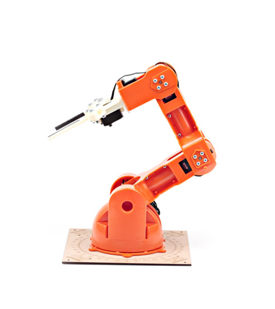
\includegraphics[width=4.0cm]{images/Bild1.png}
				\caption{Ein Roboterarm}
				
			\end{figure}
		\end{column}
	\end{columns}
\end{frame}

\subsection{Darstellung des Raums}

\begin{frame}{Darstellung des Raums}{Arbeitsraum und Konfigurationssraum}
	
	\begin{columns}
		\begin{column}[T]{0.6\textwidth}
			\begin{itemize}
				\item Der Arbeitsraum ist die Umgebung, in der sich der Roboter befindet\newline
				\item Der Konfigurationsraum ist die Menge aller seiner Konfigurationen
				\begin{itemize}[<+->]
					\item Konfiguration ist die Position des Roboters in einer für ihn verständlichen Sprache
					\item Hindernisse sind ungültige Konfigurationen
					\item Freier Raum ist die Gruppe von Konfigurationen ohne Kollisionen
					\end{itemize}
			\end{itemize}
		\end{column}
		\begin{column}[T]{0.4\textwidth}
			\begin{figure}
				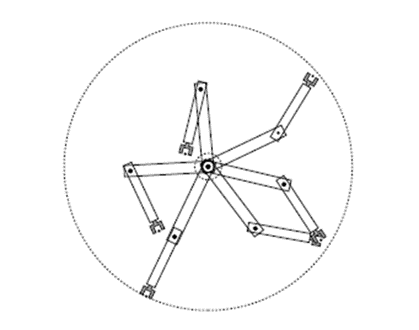
\includegraphics[width=4.5cm]{images/Bild2.png}
				\caption{Konfigurationsraum eines Roboterarms} 
			\end{figure}
		\end{column}
	\end{columns}
\end{frame}

\begin{frame}{Darstellung des Raums}{Potentialfeld}

	\begin{itemize}
		\item Punkte in dem Konfigurationsraum bekommen eine Potentialvektor
		\begin{itemize}
			\item Sie werden von Hindernisse abgestoßen
			\item Sie werden vom Ziel angezogen
			
		\end{itemize}
	\end{itemize}
	
	\begin{figure}
		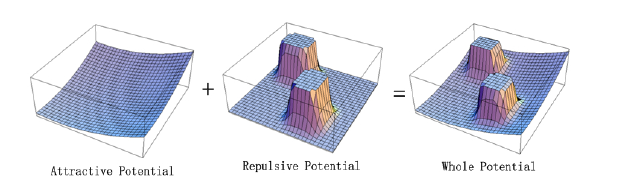
\includegraphics[width=10.5cm]{images/Potential_Field.png}
		%				\caption{Testbild in einem figure float} 
	
	\end{figure}
\end{frame}
\begin{frame}{Darstellung des Raums}{Roadmap}
	
	\begin{columns}
		\begin{column}[T]{0.6\textwidth}
			\begin{itemize}
				
				\item Die Punkte des Konfigurationsraum verbinden, um eine Roadmap zu erzeugen
				\item Bewegung in Roadmap:
				\begin{itemize}
					\item Roadmap betreten
					\item Roadmap durchlaufen
					\item Ziel erreichen
				\end{itemize}
				\item Sichtbarkeitsgraphen sind Roadmaps	
			\end{itemize}
		\end{column}
		\begin{column}[T]{0.4\textwidth}
			\begin{figure}
				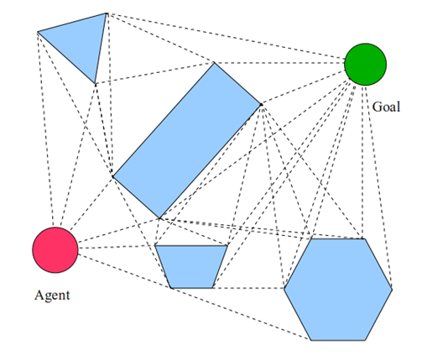
\includegraphics[width=5.5cm]{images/Bild3.png}
				\caption{Sichtbarkeitsgraph} 

			\end{figure}
		\end{column}
	\end{columns}
\end{frame}

\begin{frame}{Darstellung des Raums}{Zelldekomposition}

	\begin{itemize}
		\item Teilung des freies Raums in Zellen
		\begin{itemize}
			\item Verbindungen zwischen anliegenden Zellen speichern
		\end{itemize}
	    \item Zellen enthalten Start- und Endkonfigurationen bei der Pfadfindung.
	\end{itemize}
	
	\begin{figure}
		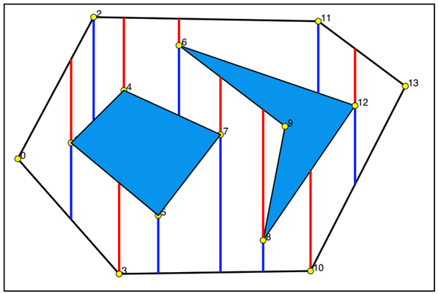
\includegraphics[width=5.0cm]{images/Bild4.png}
		\caption{Zelldekomposition mit Polygonalen Hindernissen} 

	\end{figure}
\end{frame}

\subsection{Graphen}

\begin{frame}{Graphen}{Eine Einführung}
	\begin{itemize}
		\item Graphen sind gut für Pfadfindung
		\item Ein Graph besteht aus Knoten, Kanten mit Kosten
		\item Ein gerichteter Graph unterscheidet ausgehende und eingehende Kanten
	\end{itemize}
	
	\begin{figure}
		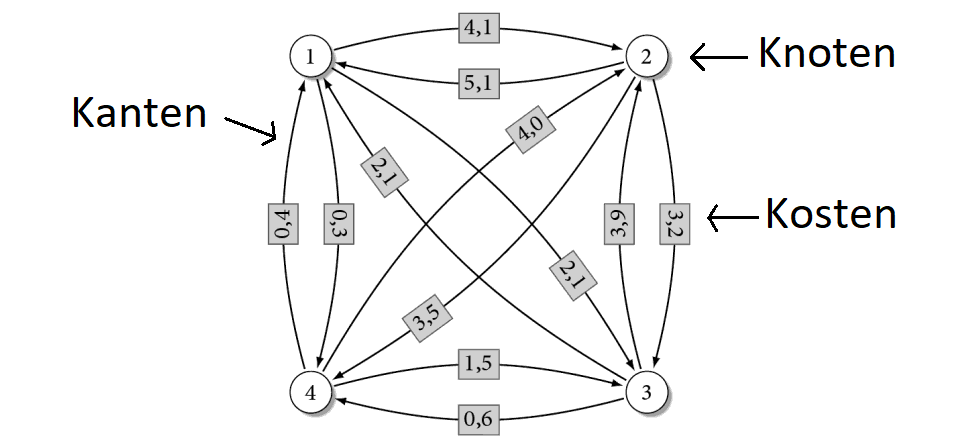
\includegraphics[width=8.0cm]{images/kk_graph_S6.png}

	\end{figure}
\end{frame}

\begin{frame}{Graphen}{Bäume}
	\begin{itemize}
		\item Hierarchische Darstellung von Graphen
		\item Ein Baum hat ein Wurzel
		\item Die Entfernung von der Wurzel ist die Tiefe des Knotens
	\end{itemize}
	
	\begin{figure}
		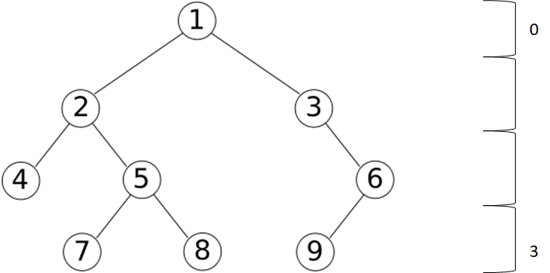
\includegraphics[width=7.0cm]{images/Bild5.png}
%		\caption{Testbild in einem figure float} 
	\end{figure}
\end{frame}
\begin{frame}{Graphen}{Navigationsnetze}
	\begin{columns}
		\begin{column}[T]{0.5\textwidth}
			\begin{itemize}
				\item Navigationsnetze definieren der freie Raum als polygonale Bereiche
				\item Verbindungen zwischen Bereichen sind im Navigationsgraph gespeichert
				\item Start und Endkonfigurationen befinden sich in den Bereichen
			\end{itemize}
		\end{column}
		\begin{column}[T]{0.5\textwidth}
			\begin{figure}
				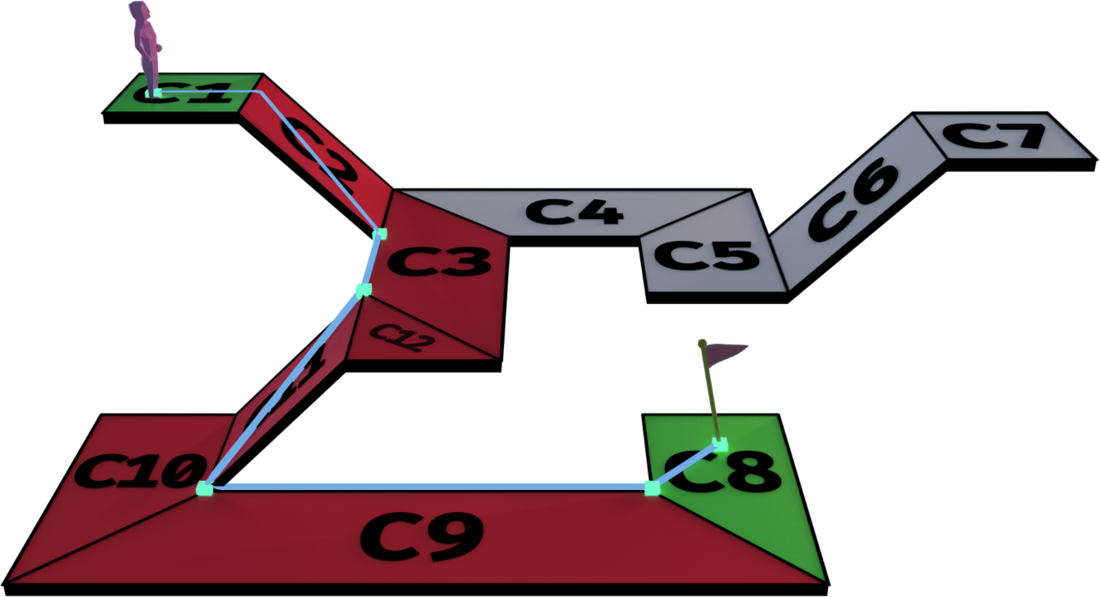
\includegraphics[width=6.5cm]{images/mesh_with_path.png}
				\caption{Navigationsnetz mit drei Ebenen} 
			\end{figure}
		\end{column}
	\end{columns}
\end{frame}

\begin{frame}{Graphen}{Rastergraphen}
	\begin{itemize}
		\item Der Konfigurationsraum wird in Feldern definiert
		\begin{itemize}
			\item Felder können verschiedene Formen haben
		\end{itemize} 
		\item Die Felder kennen ihre Nachbarn
	\end{itemize}
	\begin{figure}
		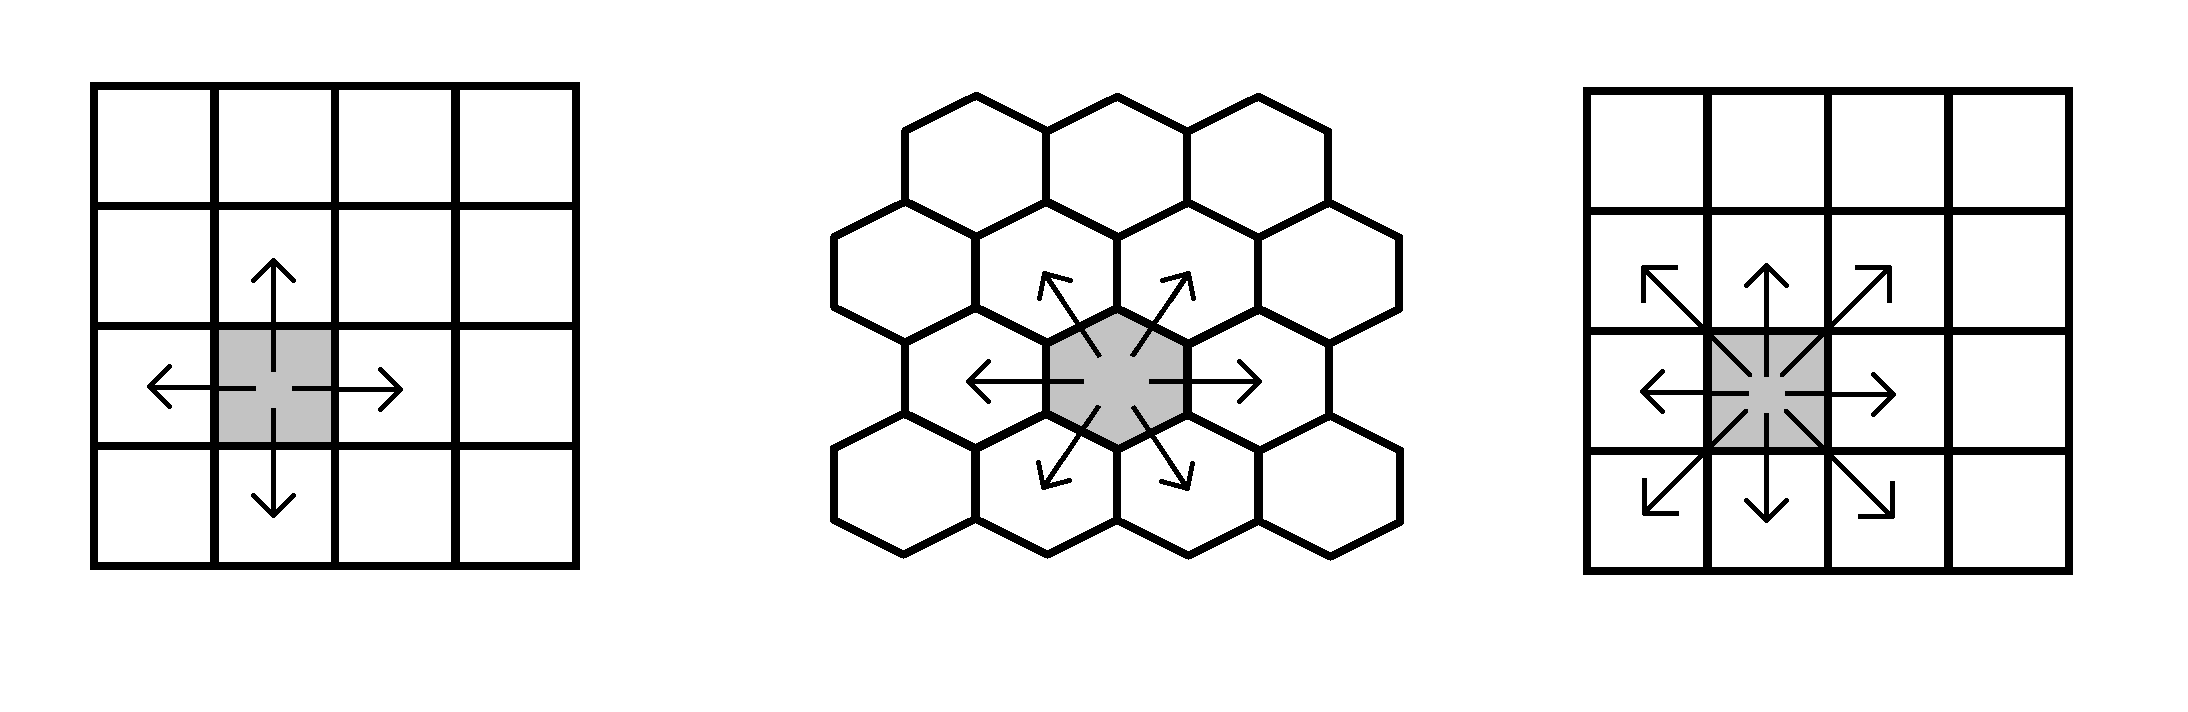
\includegraphics[width=10.0cm]{images/Grid_Tiles.png}
		\caption{Drei verschiedene Rastergraphen} 
	\end{figure}
\end{frame}

\begin{frame}{Graphen}{Sichtbarkeitsgraphen}
	\begin{columns}
		\begin{column}[T]{0.5\textwidth}
			\begin{itemize}
				\item Roadmap aus sichtbaren Punkten bilden
				\item Die Eckpunkte der Hindernisse verbinden
				\item Sensoren nehmen neue Information für den Roboter wahr, um neue  Kanten zu bilden
			\end{itemize}
		\end{column}
		\begin{column}[T]{0.5\textwidth}
			\begin{figure}
				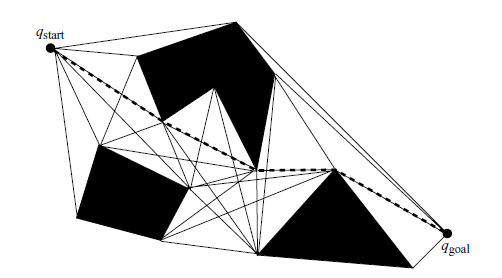
\includegraphics[width=6.5cm]{images/Robot_Motion_Visibility_Graph.png}
				\caption{Sichtbarkeitsgraph mit polygonalen Hindernissen} 
			\end{figure}
		\end{column}
	\end{columns}
\end{frame}

\section{Algorithmen zur Pfadplanung}

\begin{frame}{Gliederung der Präsentation}
	\begin{columns}[T]
		\begin{column}[T]{0.33\textwidth}
			\begin{block}{Grundlagen}
				\begin{itemize}
					\item Was ist Pfadplanung?
					\item Darstellung des Raums
					\item Graphen
					\newline\newline\newline
				\end{itemize}
			\end{block}
		\end{column}
		\begin{column}[T]{0.33\textwidth}
			\begin{block}{Algorithmen}
				\begin{itemize}
					\item Definition von Pfadplanungsalgorithmen
					\item Diskrete Pfadplanung: Beispiel Feasible Planning
					\item kontinuierliche Pfadplanung
				\end{itemize}
			\end{block}
		\end{column}
		\begin{column}[T]{0.33\textwidth}
			\begin{block}{Anwendungen}
				\begin{itemize}\color{lightgray}
					\item Rubik's Cube Rätsel
					\item Videospiele
					\item Digitales Planen von Fabrikrobotern
					\item Autonomes Fahren
					\newline\newline
				\end{itemize}		
			\end{block}
		\end{column}
	\end{columns}	
\end{frame}

\subsection{Definition von Pfadplanungsalgorithmen}
	
\begin{frame}{Algorithmen zur Pfadplanung} {Definition von Pfadplanungsalgorithmen}
	\begin{columns}
		\begin{column}[T]{0.6\textwidth}
			\begin{itemize}
				\item  Definition mit Hilfe der \textit{Church-Turing-These}
			\end{itemize}
			\begin{block}{Church-Turing-These}
				Jede im intuitiven Sinne berechenbare Funktion ist \textbf{WHILE}-berechenbar.
			\end{block}
			\begin{itemize}
				\item <2->Diese Definitionen ist Unvollständig
				\item <2->Ein Planer ist ein Algorithmus der einen Plan erstellt
				\item <2->Ein Plan kann so die Interaktion abbilden	
			\end{itemize}
		\end{column}
		\begin{column}[T]{0.4\textwidth}
			\begin{figure}
				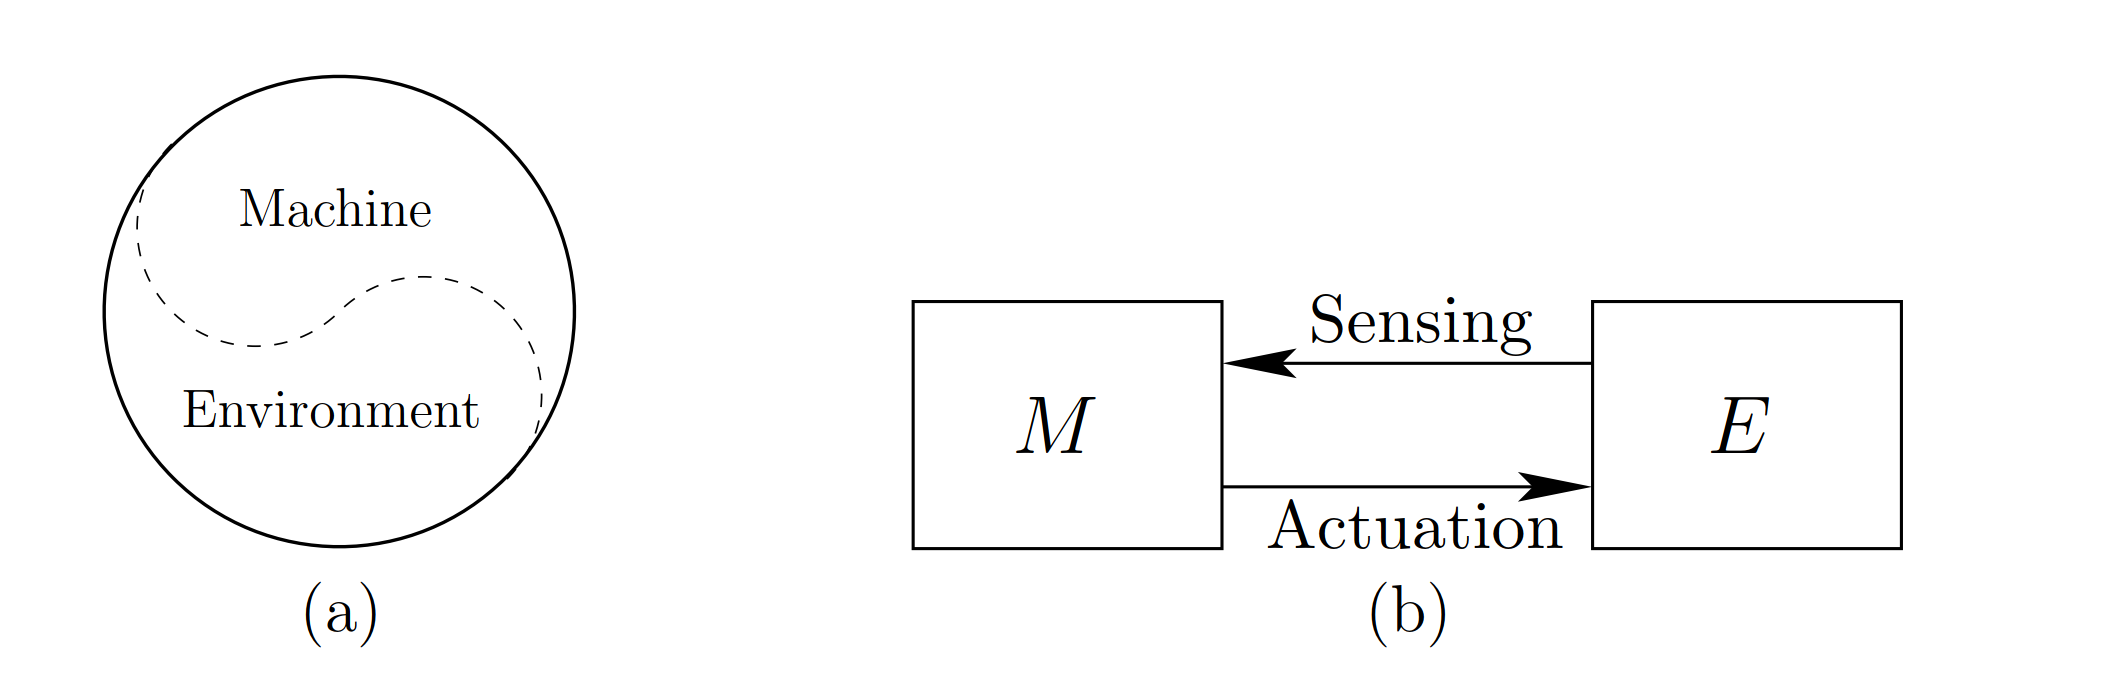
\includegraphics[width=6.5cm]{images/img224.png}
				\caption{(a) Grenze zwischen Maschine und Umgebung ist fließend.
					(b) Maschine $M$ interagiert mit der Umgebung $E$ durch Sensorik und Antrieb. } 
			\end{figure}
		\end{column}
	\end{columns}	
\end{frame}

\begin{frame}{Algorithmen zur Pfadplanung}{Verwendung des Plans}
	\only<1,2,4>{
		\begin{columns}
			\begin{column}[T]{0.3\textwidth}
				\begin{block}{Ausführen}
					\begin{itemize}
						\item mit kodierter Eingabe den Roboter programmieren
						\item Spezialmaschine für Aufgabe erstellen 
						\newline
					\end{itemize}
				\end{block}
			\end{column}
			
			\begin{column}<2->[T]{0.3\textwidth}
				\begin{block}{Verbesserung} 
					\begin{itemize}
						\item Den Plan dem Planer übergeben.
						\item Neuberechnung unter Beachtung anderer Aspekte
						\item Verbesserungs- prozess führt zum gewünschten Plan
					\end{itemize}
				\end{block}
			\end{column}
			\begin{column}<4->[T]{0.4\textwidth}
				\begin{block}{Hierarchische Inklusion}
					\begin{itemize}
						\item Plan als Teilstück eines \textit{Masterplan}
						\item Zerteilung des Problems zur leichteren Berechnung
						\item Eine Baumstruktur entsteht
						\item Mehrere Verschiebe- operationen für die Lösung erforderlich.
					\end{itemize}
				\end{block}
			\end{column}
		\end{columns}
	}
	\only<3>{
		\begin{figure}
			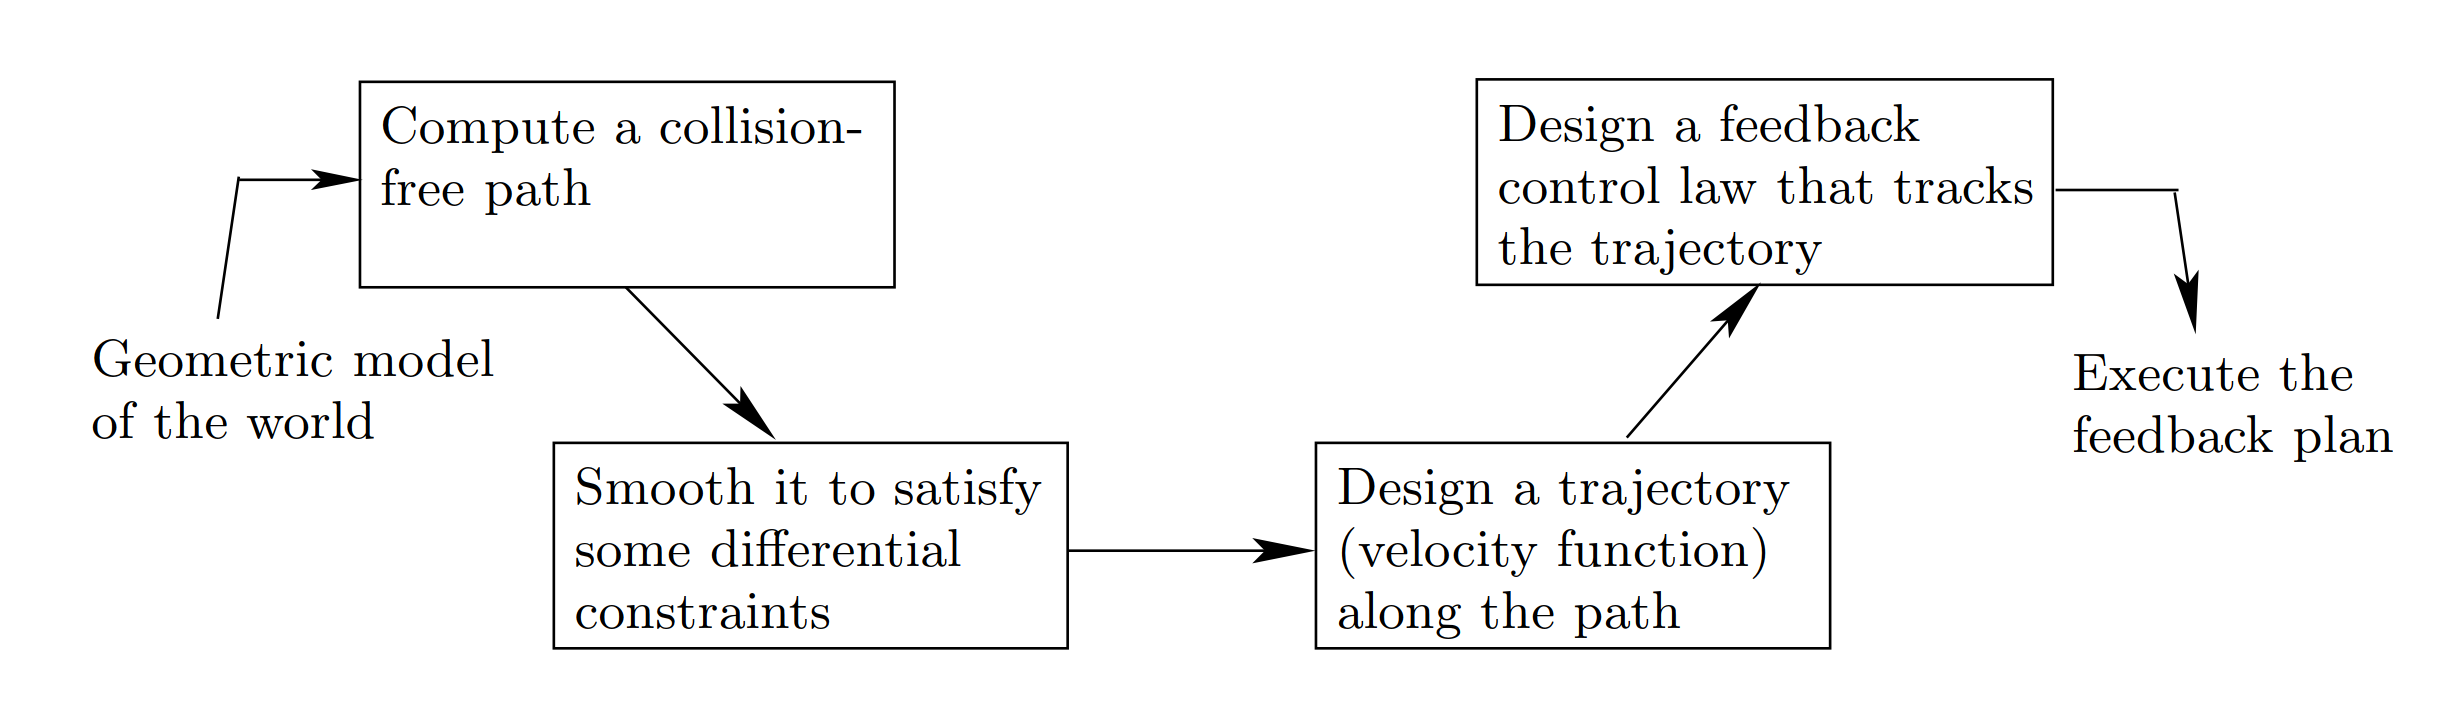
\includegraphics[width=12.5cm]{images/img247.png}
			\caption{Ein Verbesserungsprozess der sich in der Robotik bewährt hat.} 
		\end{figure}
	}	
\end{frame}

\begin{frame}{Algorithmen zur Pfadplanung}{Plan}
	\begin{figure}
		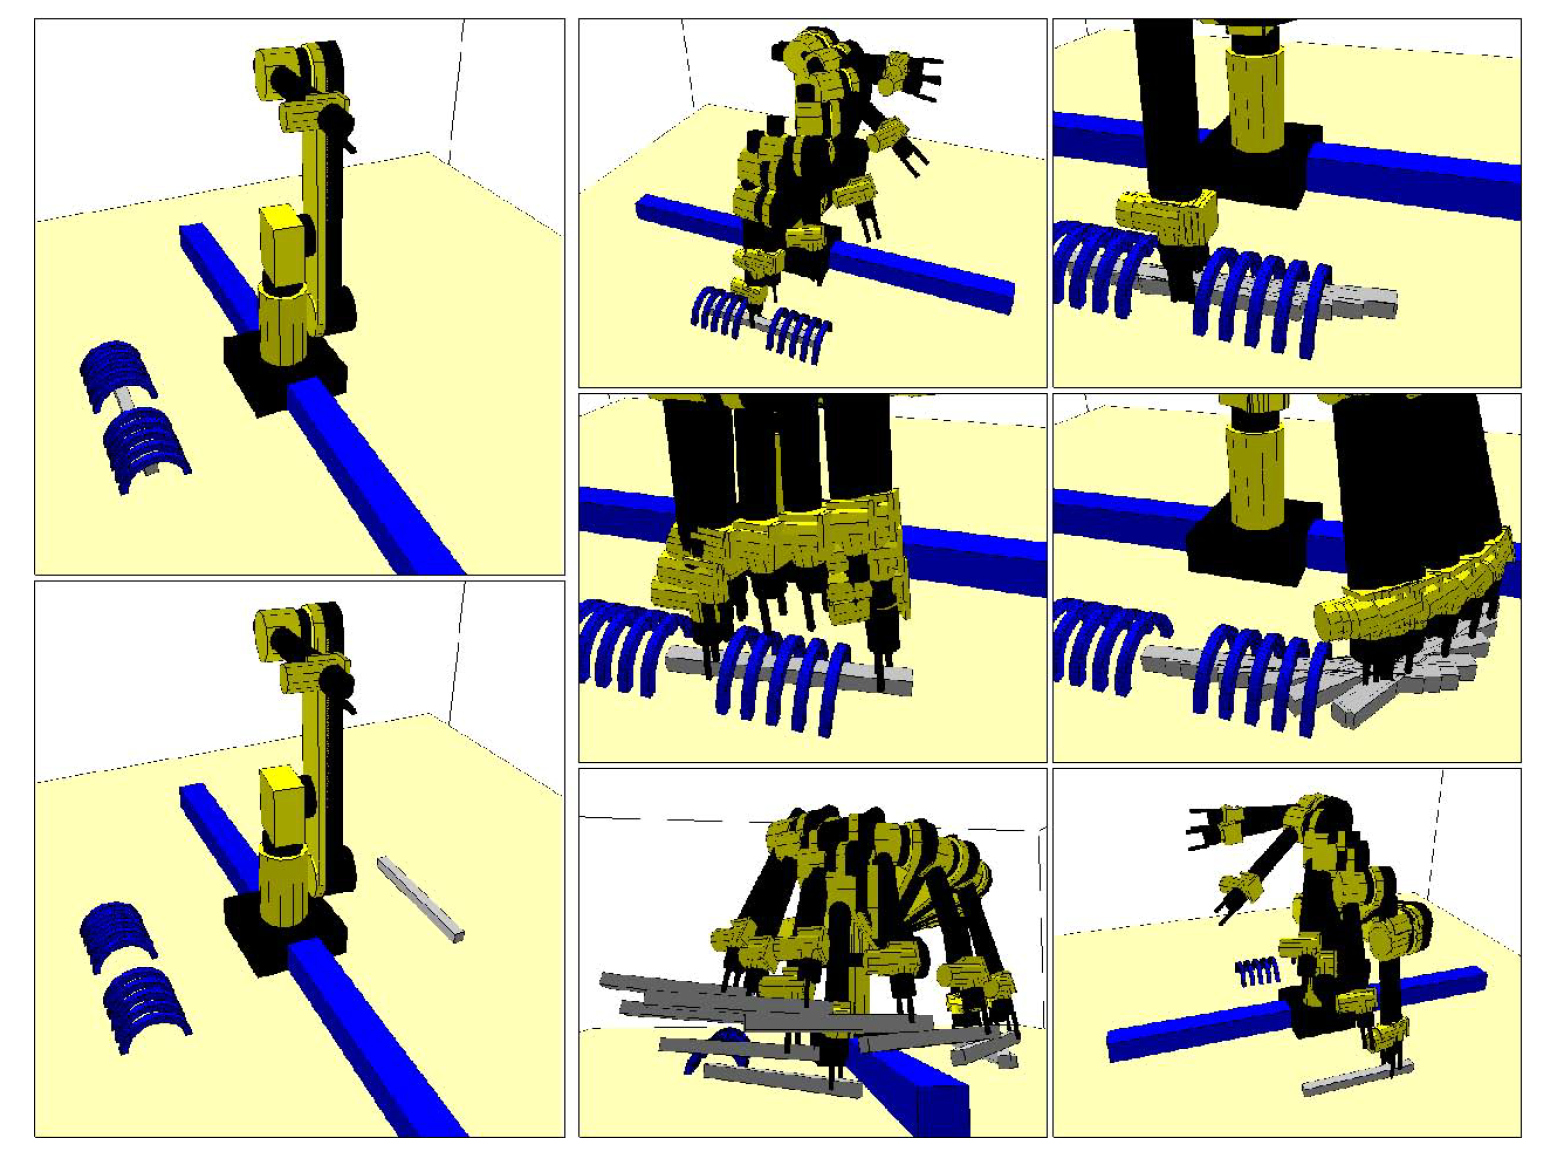
\includegraphics[width=7cm]{images/hierarchical.png}
		\caption{Roboter bewegt Stab von der Ausgangsposition zur Endposition} 
	\end{figure}
\end{frame}

\subsection{Klassifizierung von Pfadplanungsalgorithmen}

\begin{frame}{Algorithmen zur Pfadplanung}{Klassifizierung von Pfadplanungsalgorithmen}
	\begin{columns}
		\begin{column}[T]{0.5\textwidth}
			\begin{center} diskret \end{center}
			\begin{itemize}[<1->]
			\item Zustandsraum ist abzählbar unendlich 
			\item Geometrische Modelle finden keine Beachtung
			\item keine Bewegungseinschränkungen
			\item Systematisch: wenn ein Pfad existiert wird er gefunden
			\end{itemize}
		\end{column}
		\begin{column}[T]{0.5\textwidth}
			\begin{center} kontinuierlich \end{center}
				\begin{itemize}[<2>]
			\item Alle Umgebungsinformationen (Industrieroboter, kontrollierte Umgebung)
			\item Unsicherheit (Roboter mit Kameras)
			\item Bewegungseinschränkung (Roboter mit Rädern, Auto)
			\item Vorherrschaft von diskreten Algorithmen auch für konti- nuierliches Pfadplanen. 
		\end{itemize}
		\end{column}
	\end{columns}
\end{frame}

\begin{frame}{Algorithmen zur Pfadplanung}{Feasible Planning}
	\begin{itemize}
		\item Feasible Planning: ein Pfad zum Ziel wird gefunden
		\item Optimales Planen: Optimierung auf Zeit, Distanz, Anzahl Drehungen, usw.
		\begin{columns}
			\begin{column}[T]{0.5\textwidth}
				\begin{itemize}[<2>]
					\item Die Liste Q enthält den aktuellen Knoten
					\item Knoten $X_I$ ist als Startknoten gegeben
					\item Die Menge $U(x)$ enthält alle unentdeckten Knoten
					\item Die Menge $X_G$ enthält alle Zielzustände
					\item Vorgängerknoten müssen gespeichert werden
				\end{itemize}
			\end{column}
			\begin{column}[T]{0.5\textwidth}
				\begin{figure}
					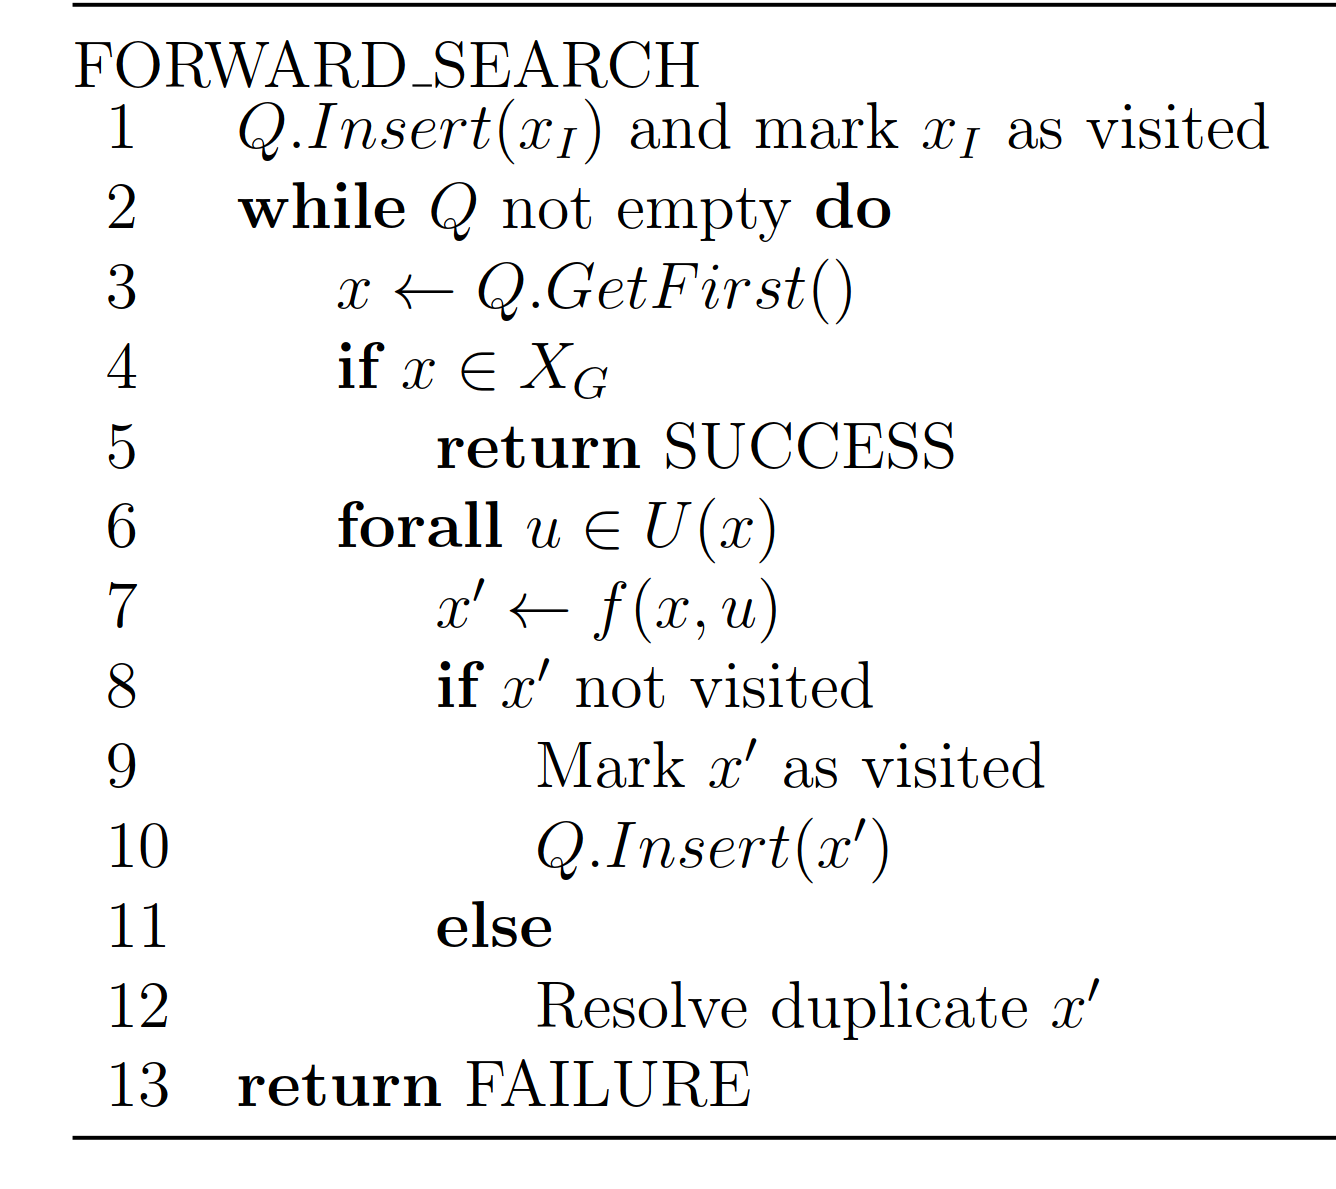
\includegraphics[width=6.0cm]{images/img225.png}
				\end{figure}
			\end{column}
		\end{columns}
	\end{itemize}
\end{frame}


\begin{frame}{Algorithmen zur Pfadplanung}{Unterscheidung von Algorithmen}
	
	\begin{center}
		Einfluss der Sortierung der Warteschlange
	\end{center}
	
	\textbf{Breadth-first Suchalgorithmus} verwendet FIFO Sortierung
	\begin{itemize}
		\item Systematisch, nicht zielgerichtet	
	\end{itemize}
	\textbf{Depht-first Suchalgorithmus} verwendet LIFO Sortierung
	\begin{itemize}
	\item teilweise systematisch, aggressive expansion, schwer kontrollierbar	
	\end{itemize}
	\textbf{Djikstra-Algorithmus} bevorzugt kleine Kantengewichte
	\begin{itemize}
		\item optimal, unnötige schritte
	\end{itemize}
	\textbf{A*-Algorithmus} schätzt Kosten zum Ziel
	\begin{itemize}
		\item optimal, zielgerichtet, schnell
	\end{itemize}	
\end{frame}

\subsection{Kontinuierliche Pfadplanung}


\begin{frame}{Algorithmen zur Pfadplanung}{Kontinuierliche Pfadplanung}
\begin{columns}
	\begin{column}[T]{0.5\textwidth}
			\begin{itemize}[<+->]
			\item Unterschiede zur diskreten Pfadplanung
			\begin{itemize}
				\item<2-> Der Zustandsraum ist überabzählbar unendlich
				\item<2-> Der Zustandsraum ist zu groß, um explizit dargestellt zu werden
			\end{itemize}
		
			\item<3-> Piano Mover's Problem
			\begin{itemize}
				\item<4-> Ein Körper muss einen kontinuierlichen Bewegungspfad finden.
				\item<4-> Geometrische Einschränkungen
				\item<4-> kein Kontakt mit Hindernissen im Raum
			\end{itemize}	
		\end{itemize}
	\end{column}
	\begin{column}[T]{0.5\textwidth}
		\begin{figure}
			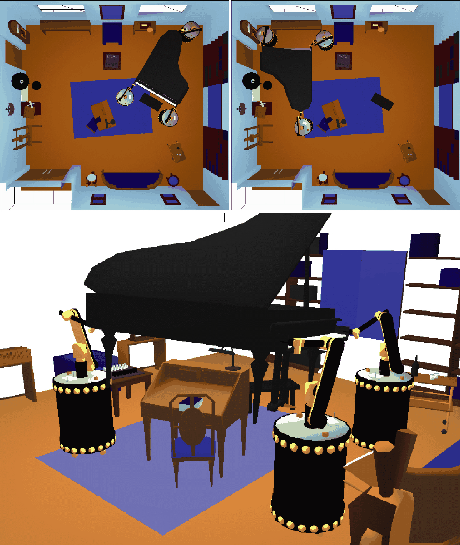
\includegraphics[width=4.0cm]{images/img233.png}
			\caption{mobile Roboter bewegen einen Flügel \cite[Abb.1.5, S.9]{Lav06}}
		\end{figure}
	\end{column}
\end{columns}
\end{frame}

\begin{frame}{Algorithmen zur Pfadplanung}{Kontinuierliche Pfadplanung}
	\begin{center}
		Zwei wichtige Motive in der Pfadplanung
	\end{center}
	\begin{columns}
		\begin{column}[T]{0.5\textwidth}<2->
			\begin{block}{Implizite Repräsentation des Zustandsraumes}
			\begin{itemize}
				\item Explizite Darstellung des Zustandsraumes nicht möglich
				\item Daher Implizite Darstellung
			\end{itemize}
			\end{block}
		\end{column}
		\begin{column}[T]{0.5\textwidth}<3->
			\begin{block}{Transformation von kontinuierlichen Modellen in diskrete}
			\begin{itemize}
				\item combinatorial motion planning
				\item sampling based motion planning
			\end{itemize}
			\end{block}
		\end{column}
	\end{columns}
\end{frame}
\begin{frame}{Gliederung der Präsentation}
	\begin{columns}[T]
		\begin{column}[T]{0.33\textwidth}
			\begin{block}{Grundlagen}
				\begin{itemize}
					\item Was ist Pfadplanung?
					\item Darstellung des Raums
					\item Graphen
					\newline\newline\newline
				\end{itemize}
			\end{block}
		\end{column}
		\begin{column}[T]{0.33\textwidth}
			\begin{block}{Algorithmen}
				\begin{itemize}
					\item Definition von Pfadplanungsalgorithmen
					\item Diskrete Pfadplanung: Beispiel Feasible Planning
					\item kontinuierliche Pfadplanung
				\end{itemize}
			\end{block}
		\end{column}
		\begin{column}[T]{0.33\textwidth}
			\begin{block}{Anwendungen}
				\begin{itemize}
					\item Rubik's Cube Rätsel
					\item Videospiele
					\item Digitales Planen von Fabrikrobotern
					\item Autonomes Fahren
					\newline\newline
				\end{itemize}		
			\end{block}
		\end{column}
	\end{columns}	
\end{frame}
\section{Anwendungen der Pfadplanungs}
\subsection{Rubic's Cube Rätsel}
\begin{frame}{Anwendungen der Pfadplanung}{Das Rubic's Cube Rätsel}
	\begin{columns}
		\begin{column}[T]{0.5\textwidth}
				\begin{itemize}[<+->]
					\item Zustandsraum: Alle möglichen Farbverteilungen
					\item Aktionsrahmen: Die Menge aller möglichen Drehungen
					\item bestmöglicher Pfad: die geringste Anzahl an Drehungen, bis der Würfel einfarbige Seiten hat
					\item diskret
				\end{itemize}
		\end{column}
		\begin{column}[T]{0.5\textwidth}
			\begin{figure}
				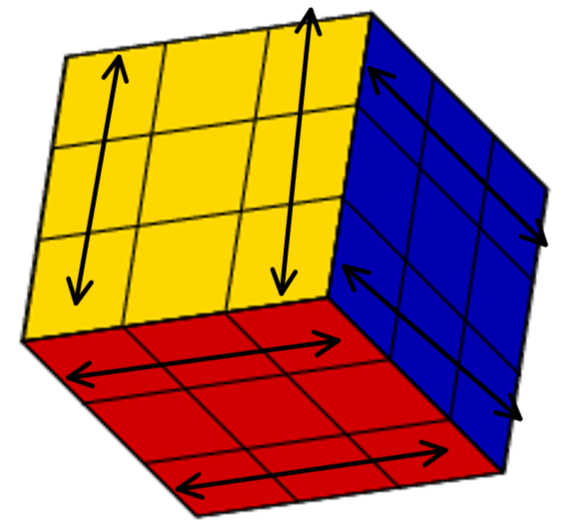
\includegraphics[width=4.5cm]{images/img229_a.png}
				\caption{Der Rubik's Cube und sein Aktionsrahmen }
			\end{figure}
		\end{column}
	\end{columns}
\end{frame}
\subsection{Videospiele}
\begin{frame}{Anwendungen der Pfadplanung}{Videospiele}
	\begin{columns}
		\begin{column}[T]{0.5\textwidth}
			\begin{itemize}[<+->]
				\item Zustandsraum: Alle möglichen Positionen der zu bewegenden Einheit und alle möglichen Map-Gegebenheiten
				\item Aktionsrahmen: alle möglichen Bewegungsrichtungen
				\item bestmöglicher Pfad: der schnellste Weg um Ziel
				\item diskret
			\end{itemize}
		\end{column}
		\begin{column}[T]{0.5\textwidth}
			\begin{figure}
				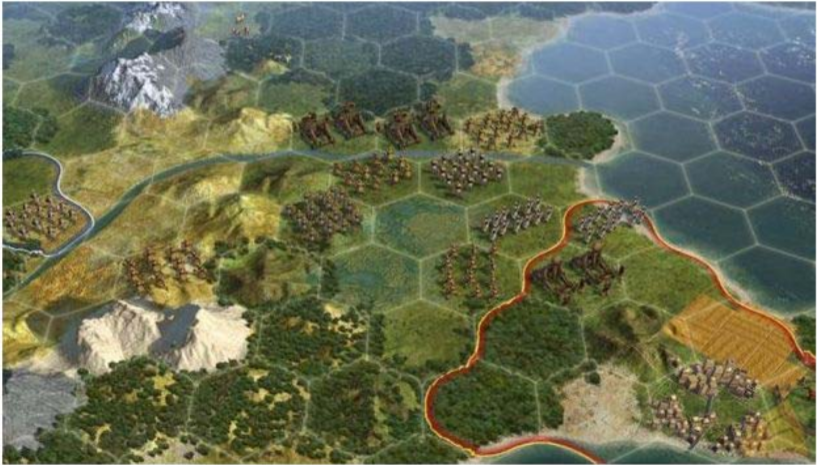
\includegraphics[width=6.0cm]{images/Civ5.png}
				\caption{Screenshot aus Civilisation V}
			\end{figure}
		\end{column}
	\end{columns}
\end{frame}
\subsection{Digitales Planen von Fabrikrobotern}
\begin{frame}{Anwendungen der Pfadplanung}{Digitales Planen von Fabrikrobotern}
	\begin{columns}
		\begin{column}[T]{0.5\textwidth}
			\begin{itemize}[<+->]
				\item Zustandsraum: Alle möglichen Position der Fabrikroboter, des Autos und des zu montierenden Teils
				\item Aktionsrahmen: Die Menge aller möglichen Bewegungen des Roboters
				\item kontinuierlich
				\item Alle Umgebungsinformationen sind bekannt
			\end{itemize}
		\end{column}
		\begin{column}[T]{0.5\textwidth}
			\begin{figure}
				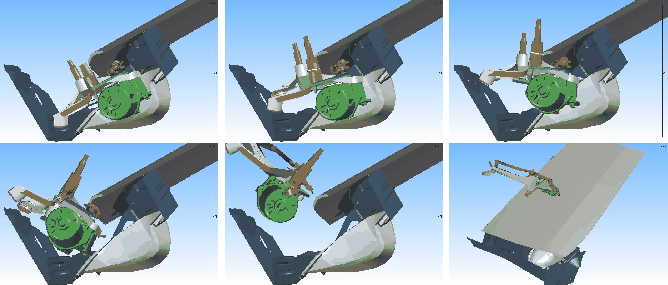
\includegraphics[width=7.0cm]{images/img231.png}
				\caption{Scheibenwischer wird an Auto angebracht} 
			\end{figure}
		\end{column}
	\end{columns}
\end{frame}
\subsection{Autonomes Fahren}
\begin{frame}{Anwendungen der Pfadplanung}{Autonomes Fahren}
	\begin{columns}
		\begin{column}[T]{0.6\textwidth}
			\begin{itemize}[<+->]
				\item Zustandsraum: Jede mögliche Position auf der Welt und jede mögliche Umgebung
				\item Aktionsrahmen:
				\begin{itemize}[<2->]
					\item Beschleunigen
					\item Bremsen
					\item Lenken
					\item blinken
					\item Gang wechseln		
				\end{itemize}
				\item kontinuierlich
				\item Planung mit Ungewissheit
				\item Planung mit Bewegungseinschränkungen
			\end{itemize}
		\end{column}
		\begin{column}[T]{0.4\textwidth}
			\begin{figure}
				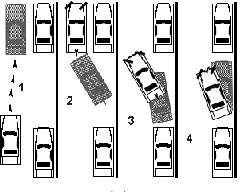
\includegraphics[width=6.0cm]{images/img239.png}
				\caption{Autonomes Einparken} 
			\end{figure}
		\end{column}
	\end{columns}
\end{frame}

\begin{frame}
\begin{center}
\huge Danke für eure Aufmerksamkeit!
\end{center}

\begin{figure}
	
\includegraphics[width=4.0cm]{images/smiley.jpg}
	
\end{figure}
\begin{center}
	Fragen gerne im Forum stellen!
\end{center}
\end{frame}


\end{document}
